%%%%%%%%%%%%%%%%%%%%%%%%%%%%%%%%%%%%%%%%%%%%%%%%%%%%%%%%%%%%%%%%%%%%%%%%%%%%%%
% CS110: Introduction to Computing
% Copyright 2015 Pejman Ghorbanzade <mail@ghorbanzade.com>
% Creative Commons Attribution-ShareAlike 4.0 International License
% https://github.com/ghorbanzade/UMB-CS110-2015S/blob/master/LICENSE
%%%%%%%%%%%%%%%%%%%%%%%%%%%%%%%%%%%%%%%%%%%%%%%%%%%%%%%%%%%%%%%%%%%%%%%%%%%%%%

\def \topDirectory {../..}
\def \texDirectory {\topDirectory/src/main/tex}

\documentclass[10pt, compress]{beamer}

\usepackage{\texDirectory/template/style/directives}
%%%%%%%%%%%%%%%%%%%%%%%%%%%%%%%%%%%%%%%%%%%%%%%%%%%%%%%%%%%%%%%%%%%%%%%%%%%%%%
% CS110: Introduction to Computing
% Copyright 2015 Pejman Ghorbanzade <mail@ghorbanzade.com>
% Creative Commons Attribution-ShareAlike 4.0 International License
% https://github.com/ghorbanzade/UMB-CS110-2015S/blob/master/LICENSE
%%%%%%%%%%%%%%%%%%%%%%%%%%%%%%%%%%%%%%%%%%%%%%%%%%%%%%%%%%%%%%%%%%%%%%%%%%%%%%

\course{id}{CS110}
\course{name}{Introduction to Computing}
\course{venue}{Tue/Thu, 5:30 PM - 6:45 PM}
\course{semester}{Spring 2015}
\course{department}{Department of Computer Science}
\course{university}{University of Massachusetts Boston}

\instructor{name}{Pejman Ghorbanzade}
\instructor{title}{}
\instructor{position}{Student Instructor}
\instructor{email}{pejman@cs.umb.edu}
\instructor{phone}{617-287-6419}
\instructor{office}{S-3-124B}
\instructor{office-hours}{Tue/Thu 19:00-20:30}
\instructor{address}{University of Massachusetts Boston, 100 Morrissey Blvd., Boston, MA}

\usepackage{\texDirectory/template/style/beamerthemeUmassLecture}
\doc{number}{15}
%\setbeamertemplate{footline}[text line]{}

\begin{document}
\prepareCover

\section{Course Administration}

\begin{frame}[fragile]
\frametitle{Course Administration}
Assignment 5 Released. Due on April 30, 2015 at 17:30 PM.
Quiz 4 Released. Due on April 24, 2015 at 11:00 PM.
Assignment 6 Released. Submission Optional. Due on May 14, 2015.
\end{frame}

\begin{frame}[fragile]
	\frametitle{Overview}
	\begin{itemize}
		\item[] Exception Handling
		\begin{itemize}
			\item[] Motivation
			\item[] Introduction
			\item[] Handling Exceptions
			\item[] Throwing Exceptions
		\end{itemize}
	\end{itemize}
\end{frame}

\plain{}{Exception Handling}

\section{Motivation}

\begin{frame}[fragile]
	\frametitle{Exception Handling}
	\begin{block}{Objective}
		Write a program \texttt{ExceptionTest.java} that asks a number $x$ from user and prints $x+2$ as output.
	\end{block}
\end{frame}

\begin{frame}[fragile]
	\frametitle{Exception Handling}
	\begin{block}{Class \texttt{ExceptionTest.java} (v1.0)}
		\begin{minted}[fontsize=\small,tabsize=8,linenos,firstnumber=1]{java}
import java.util.Scanner;
public class ExceptionTest {
	public static void main(String[] args) {
		Scanner input = new Scanner(System.in);
		System.out.print("Enter number: ");
		int num = input.nextInt();
		input.close();
		System.out.println("Result is: "+ (num+2));
	}
}
		\end{minted}
	\end{block}
\end{frame}

\begin{frame}[fragile]
	\frametitle{Exception Handling}
	\begin{block}{Problem Statement}
		What if the user enters a string instead of a number?
\begin{verbatim}
	> javac ExceptionTest.java
	> java ExceptionTest
		Enter number: 5
		Result is: 7
	> java ExceptionTest
		Enter number: Evil
		Exception in thread "main"
			java.lang.NumberFormatException:
			For input string: "hi".
\end{verbatim}
	\end{block}
\end{frame}

\begin{frame}[fragile]
	\frametitle{Exception Handling}
	\begin{block}{Proposed Solution}
		Provide means to resolve, within the program, anomalous conditions that may interrupt normal flow of program execution.
	\end{block}
	\begin{block}{Advantage}
		Maintain normal flow of the application in the event of exception.
	\end{block}
\end{frame}

\begin{frame}[fragile]
	\frametitle{Exception Handling}
	\begin{figure}
		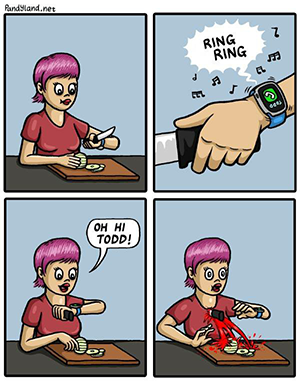
\includegraphics[height=0.8\textheight]{\texDirectory/template/images/cartoon.png}
	\end{figure}
\end{frame}

\section{Introduction}

\begin{frame}[fragile]
	\frametitle{Exception Handling}
	\begin{block}{Definition}
		Exception is an object thrown by the method in which an error has occurred. Thrown objects are handed off to the runtime system to be treated by an \textbf{exception handler}.
	\end{block}
\end{frame}

\begin{frame}[fragile]
	\frametitle{Exception Handling}
	\begin{block}{Definition}
		Exception handler is a block of code in a method that is executed once the method \textbf{catches} exception objects of an Exception class.
	\end{block}
\end{frame}

\begin{frame}[fragile]
	\frametitle{Exception Handling}
	\begin{block}{Hierarchy of Exceptions}
		\begin{figure}
			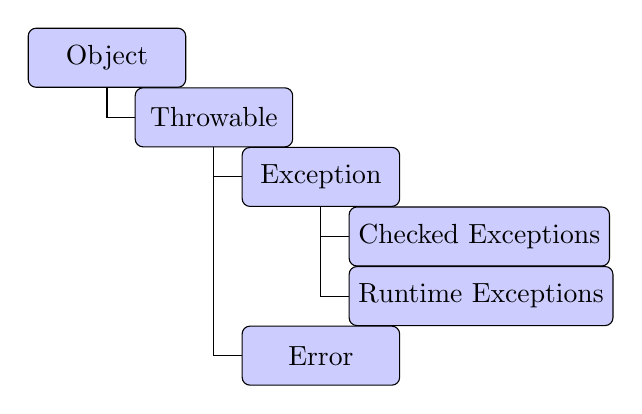
\begin{tikzpicture}[
				cell/.style={rectangle, draw, fill=blue!20, rounded corners=1mm, minimum width=2cm, minimum height=7.5mm},
				grandchild/.style={grow=down,xshift=1em,anchor=west, edge from parent path={(\tikzparentnode.south) |- (\tikzchildnode.west)}},
				first/.style={level distance=5ex},
				second/.style={level distance=10ex},
				third/.style={level distance=15ex},
				fourth/.style={level distance=20ex}
				]
				\coordinate
				child[level distance=0mm] {
				node[cell, anchor=east] {Object}
					child[grandchild, first] {
						node[cell] {Throwable}
						child[grandchild, first] {
							node[cell] {Exception}
							child[grandchild, first] {
								node[cell, first] {Checked Exceptions}
							}
							child[grandchild, second] {
								node[cell, first] {Runtime Exceptions}
							}
						}
						child[grandchild, fourth] {
							node[cell] {Error}
						}
					}
				};
			\end{tikzpicture}
		\end{figure}
	\end{block}
\end{frame}

\begin{frame}[fragile]
	\frametitle{Exception Handling}
	\begin{block}{Checked Exceptions}
		Checked expections are exceptional conditions that \alert{must} be caught in the method or thrown by the method, for a program to compile.
	\end{block}
	\begin{block}{Examples}
		\begin{itemize}
			\item[] IOException
			\item[] SQLException
			\item[] DataAccessException
			\item[] ClassNotFoundException
		\end{itemize}
	\end{block}
\end{frame}

\begin{frame}[fragile]
	\frametitle{Exception Handling}
	\begin{block}{Errors}
		Errors are exceptional conditions, caused by a problem external to the application, that \alert{should not} be caught or thrown. Errors are irrecoverable and in the rare event of occurrence, should interrupt the control flow.
	\end{block}
	\begin{block}{Examples}
		\begin{itemize}
			\item[] OutOfMemoryError
			\item[] VirtualMachineError
			\item[] ThreadDeath
			\item[] FactoryConfigurationError
		\end{itemize}
	\end{block}
\end{frame}

\begin{frame}[fragile]
	\frametitle{Exception Handling}
	\begin{block}{Runtime Exceptions}
		Runtime exceptions are exceptional conditions internal to the application, that the compiler cannot anticipate. Runtime exceptions \alert{should be} caught within the method body to maintain control flow once they occur.
	\end{block}
	\begin{block}{Examples}
		\begin{itemize}
			\item[] ArithmeticException
			\item[] NullPointerException
			\item[] IndexOutOfBoundsException
			\item[] NumberFormatException
		\end{itemize}
	\end{block}
\end{frame}

\section{Handling Exceptions}

\begin{frame}[fragile]
	\frametitle{Exception Handling}
	\begin{block}{Objective}
		Write a program \texttt{ExceptionTest.java} that asks a number $x$ from user and prints $x+2$ as output.
	\end{block}
\end{frame}

\begin{frame}[fragile]
	\frametitle{Exception Handling}
	\begin{block}{Class \texttt{ExceptionTest.java} (v1.0)}
		\begin{minted}[fontsize=\small,tabsize=8,linenos,firstnumber=1]{java}
import java.util.Scanner;
public class ExceptionTest {
	public static void main(String[] args) {
		Scanner input = new Scanner(System.in);
		System.out.print("Enter number: ");
		int num = input.nextInt();
		input.close();
		System.out.println("Result is: "+ (num+2));
	}
}
		\end{minted}
	\end{block}
\end{frame}

\begin{frame}[fragile]
	\frametitle{Exception Handling}
	\begin{block}{Problem Statement}
		\begin{itemize}
			\item[] What if the user enters a String?
		\end{itemize}
	\end{block}
	\begin{block}{Proposed Solution}
		Ask the program to \alert{try} to ask a number from user. In case an exception occurred, ask the program to \alert{catch} and handle it.
	\end{block}
\end{frame}

\begin{frame}[fragile]
	\frametitle{Exception Handling}
	\begin{block}{Class \texttt{ExceptionTest.java} (v2.0)}
		\begin{minted}[fontsize=\small,tabsize=8,linenos,firstnumber=1]{java}
import java.util.InputMismatchException;
import java.util.Scanner;
public class ExceptionTest {
	public static void main(String[] args) {
		Scanner input = new Scanner(System.in);
		System.out.print("Enter number: ");
		try {
			int num = input.nextInt();
			System.out.println("Result is: "+ (num+2));
		}
		catch (InputMismatchException e) {
			System.out.println("Input not a number.");
		}
		input.close();
	}
}
		\end{minted}
	\end{block}
\end{frame}

\begin{frame}[fragile]
	\frametitle{Exception Handling}
	\begin{block}{Try Block}
		Try block contains the statements that may cause an exception. Once an exception is \alert{thrown}, execution of the try block is terminated.
	\end{block}
	\begin{block}{Catch Block}
		Catch block contains the statements to be executed in the event of an exception \alert{of similar type}, in its corresponding try block.
	\end{block}
\end{frame}

\begin{frame}[fragile]
	\frametitle{Exception Handling}
	\begin{block}{Syntax Structure}
		\begin{minted}[fontsize=\small,tabsize=8,linenos=none,firstnumber=1]{java}
try {
	// statements that may cause an exception
}
catch (ExceptionType e) {
	// statements to handle the exception
}
		\end{minted}
	\end{block}
\end{frame}

\begin{frame}[fragile]
	\frametitle{Exception Handling}
	\begin{block}{Remember}
		\begin{itemize}
			\item[] Catch block must always follow a try block.
			\item[] A try block can have multiple catch blocks of different types.
			\item[] Exception is caught by the first catch block of same type.
			\item[] Normal flow of program continues after catch block is executed.
			\item[] It is a bad practice to leave a catch block empty.
		\end{itemize}
	\end{block}
\end{frame}

\begin{frame}[fragile]
	\frametitle{Exception Handling}
	\begin{block}{Problem Statement}
		What happens if the exception is not caught within catch blocks?
	\end{block}
	\begin{block}{Solution}
		JVM searches in \alert{Call Stack} for catch blocks with similar ExceptionType. If no handler is found, the runtime terminates.
	\end{block}
\end{frame}

\begin{frame}[fragile]
	\frametitle{Exception Handling}
	\begin{block}{Problem Statement}
		What happens if the exception is not caught within catch blocks?
	\end{block}
	\begin{block}{Solution}
		If the exception is thrown by the method, JVM searches in \alert{Call Stack} for catch blocks with similar ExceptionType. If no handler is found, the runtime terminates.
	\end{block}
\end{frame}

\begin{frame}[fragile]
	\frametitle{Exception Handling}
	\begin{block}{Call Stack}
		Call stack is the ordered list of methods called in runtime, starting from main method and ending with the method whose statements are being executed.
	\end{block}
\end{frame}

\begin{frame}[fragile]
	\frametitle{Exception Handling}
	\begin{block}{Objective}
		Write a program \texttt{ExceptionTest2.java} that asks a number $x$ from user and prints ``invalid input'' for all improper inputs and	$10/x$ otherwise.
	\end{block}
\end{frame}

\begin{frame}[fragile]
	\frametitle{Exception Handling}
	\begin{block}{Class \texttt{ExceptionTest2.java} (v1.0)}
		\begin{minted}[fontsize=\small,tabsize=8,linenos,firstnumber=1]{java}
import java.util.Scanner;
public class ExceptionTest {
	public static void main(String[] args) {
		Scanner input = new Scanner(System.in);
		System.out.print("Enter number: ");
		int num = input.nextInt();
		int double result = 10/num;
		System.out.println("Result is: "+ result);
		input.close();
	}
}
		\end{minted}
	\end{block}
\end{frame}

\begin{frame}[fragile]
	\frametitle{Exception Handling}
	\begin{block}{Class \texttt{ExceptionTest2.java} (v2.0) (Page 1)}
		\begin{minted}[fontsize=\small,tabsize=8,linenos,firstnumber=1]{java}
import java.util.InputMismatchException;
import java.util.ArithmeticException;
import java.util.Scanner;
public class ExceptionTest {
	public static void main(String[] args) {
		Scanner input = new Scanner(System.in);
		System.out.print("Enter number: ");
		\end{minted}
	\end{block}
\end{frame}

\begin{frame}[fragile]
	\frametitle{Exception Handling}
	\begin{block}{Class \texttt{ExceptionTest2.java} (v2.0) (Page 2)}
		\begin{minted}[fontsize=\small,tabsize=8,linenos,firstnumber=8]{java}
		try {
			int num = input.nextInt();
			double result = 10/num;
			System.out.println("Result is: "+ result);
		}
		catch (InputMismatchException e) {
			System.out.println("Invalid input.");
		}
		catch (ArithmeticException e) {
			System.out.println("Invalid input.");
		}
		input.close();
	}
}
		\end{minted}
	\end{block}
\end{frame}

\begin{frame}[fragile]
	\frametitle{Exception Handling}
	\begin{block}{Problem Statement}
		Redundant catch blocks for different exceptions.
	\end{block}
	\begin{block}{Proposed Solution}
		\begin{minted}[fontsize=\small,tabsize=8,linenos,firstnumber=13]{java}
		catch (InputMismatchException|ArithmeticException e) {
			System.out.println("Invalid input.");
		}
		\end{minted}
	\end{block}
\end{frame}

\begin{frame}[fragile]
	\frametitle{Exception Handling}
	\begin{block}{Problem Statement}
		What happens if an unknown exception occurs?
	\end{block}
	\begin{block}{Possible Solution}
		\begin{minted}[fontsize=\small,tabsize=8,linenos,firstnumber=13]{java}
		catch (Exception e) {
			System.out.println("Invalid input.");
		}
		\end{minted}
	\end{block}
	\begin{block}{Caution}
		\begin{itemize}
			\item[] Treating all exceptions alike is discouraged.
			\item[] Using \texttt{catch(Throwable e)} is \alert{extremely} discouraged.
		\end{itemize}
	\end{block}
\end{frame}

\begin{frame}[fragile]
	\frametitle{Exception Handling}
	\begin{block}{Nested Try-Catch Blocks}
		It is possible to have a try-catch block inside another try-catch block. Exception \alert{not} handled in child block will be treated as exception for the parent block.
	\end{block}
\end{frame}

\begin{frame}[fragile]
	\frametitle{Exception Handling}
	\begin{block}{Finally Block}
		Finally block contains statements to be executed \alert{regardless} of whether or not an exception occurs within the try block.

		Finally block is executed even in presence of control transfer statements (\texttt{return}, \texttt{continue} or \texttt{break}) in try or catch blocks. This provides good opportunity to use cleanup codes within the finally block.
	\end{block}
\end{frame}

\section{Throwing Exceptions}

\begin{frame}[fragile]
	\frametitle{Exception Handling}
	\begin{block}{Objective}
		Write a program \texttt{CarTest.java} that using a class \texttt{Car.java} asks the user for the number of people to get on board a car \texttt{car1}.
	\end{block}
\end{frame}

\begin{frame}[fragile]
	\frametitle{Exception Handling}
	\begin{block}{\texttt{Car.java} (v1.0) (Page 1)}
		\begin{minted}[fontsize=\small,tabsize=8,linenos,firstnumber=1]{java}
import java.util.InputMismatchException;
import java.util.Scanner;
public class Car {
	private int numPassengerMax;
	private int numPassenger;
	public Car(int numPassengerMax) {
		this.numPassenger = numPassengerMax;
	}
	public int getNumPassenger() {
		return numPassenger;
	}
		\end{minted}
	\end{block}
\end{frame}

\begin{frame}[fragile]
	\frametitle{Exception Handling}
	\begin{block}{\texttt{Car.java} (v1.0) (Page 2)}
		\begin{minted}[fontsize=\small,tabsize=8,linenos,firstnumber=12]{java}
	public void board() {
		System.out.print("How many people to board? ");
		Scanner input = new Scanner(System.in);
		try {
			int num = input.nextInt();
			if (numPassenger + num <= numPassengerMax)
				numPassenger += num;
			else
				System.out.println("Exceeds seating capacity");
		}
		\end{minted}
	\end{block}
\end{frame}

\begin{frame}[fragile]
	\frametitle{Exception Handling}
	\begin{block}{\texttt{Car.java} (v1.0) (Page 3)}
		\begin{minted}[fontsize=\small,tabsize=8,linenos,firstnumber=22]{java}
		catch (InputMismatchException e) {
			System.out.println("Invalid input.");
		}
		catch (Exception e) {
			System.out.println("Bad response.");
		}
		finally {
			input.close();
		}
	}
}
		\end{minted}
	\end{block}
\end{frame}

\begin{frame}[fragile]
	\frametitle{Exception Handling}
	\begin{block}{\texttt{CarTest.java} (v1.0)}
		\begin{minted}[fontsize=\small,tabsize=8,linenos,firstnumber=1]{java}
public class CarTest {
	public static void main(String[] args) {
		Car car1 = new Car(4);
		car1.board();
	}
}
		\end{minted}
	\end{block}
	\begin{block}{Output}
\begin{verbatim}
	How many people to board? some word
	Invalid Input
	How many people to board? 5
	Exceeds seating capacity
\end{verbatim}
	\end{block}
\end{frame}

\begin{frame}[fragile]
	\frametitle{Exception Handling}
	\begin{block}{Definition}
		A method is free not to catch an Exception but rather hand it to a parent method. In this case, the method \alert{throws} the exception. A method can only throw exceptions that it specifies.
	\end{block}
\end{frame}

\begin{frame}[fragile]
	\frametitle{Exception Handling}
	\begin{block}{Throwables}
		Exceptions are thrown by
		\begin{itemize}
			\item[] Methods developed by programmer
			\item[] Methods in pre-developed packages
			\item[] Java Runtime Environment
		\end{itemize}
		All exceptions thrown are objects of class \texttt{Throwable}.
	\end{block}
\end{frame}

\begin{frame}[fragile]
	\frametitle{Exception Handling}
	\begin{block}{\texttt{throws} keyword}
		A method can specify type of exceptions that it might throw without catching, to the call stack by using the \texttt{throws} keyword in its method declaration.
	\end{block}
	\begin{block}{Syntax}
		\begin{minted}[fontsize=\small,tabsize=8,linenos,firstnumber=12]{java}
public void board() throws InputMismatchException {
	// method body
}
		\end{minted}
	\end{block}
\end{frame}

\begin{frame}[fragile]
	\frametitle{Exception Handling}
	\begin{block}{Chaining Exceptions}
		A method throwing an exception declares itself prone to exceptions. In case an exception occurs (whose type matches types of exceptions thrown by the method), Java Runtime Environment expects the parent method to handle the exception.
	\end{block}
\end{frame}

\begin{frame}[fragile]
	\frametitle{Exception Handling}
	\begin{block}{\texttt{Car.java} (v2.0) (Page 1)}
		\begin{minted}[fontsize=\small,tabsize=8,linenos,firstnumber=1]{java}
import java.util.Scanner;
public class Car {
	private int numPassengerMax;
	private int numPassenger;
	public Car(int numPassengerMax) {
		this.numPassenger = numPassengerMax;
	}
	public int getNumPassenger() {
		return numPassenger;
	}
		\end{minted}
	\end{block}
\end{frame}

\begin{frame}[fragile]
	\frametitle{Exception Handling}
	\begin{block}{\texttt{Car.java} (v2.0) (Page 2)}
		\begin{minted}[fontsize=\small,tabsize=8,linenos,firstnumber=11]{java}
	public void board() {
	public void board() {
		System.out.print("How many people to board? ");
		Scanner input = new Scanner(System.in);
		int num = input.nextInt();
		if (numPassenger + num <= numPassengerMax)
			numPassenger += num;
		else
			System.out.println("Exceeds seating capacity");
		input.close();
	}
}
		\end{minted}
	\end{block}
\end{frame}

\begin{frame}[fragile]
	\frametitle{Exception Handling}
	\begin{block}{\texttt{CarTest.java} (v2.0)}
		\begin{minted}[fontsize=\small,tabsize=8,linenos,firstnumber=1]{java}
import java.util.InputMismatchException;
public class CarTest {
	public static void main(String[] args) {
		Car car1 = new Car(4);
		try {
			car1.board();
		}
		catch (InputMismatchException e) {
			System.out.println("Invalid input.");
		}
		catch (Exception e) {
			System.out.println("Bad response.");
		}
	}
}
		\end{minted}
	\end{block}
\end{frame}

\begin{frame}[fragile]
	\frametitle{Exception Handling}
	\begin{figure}
		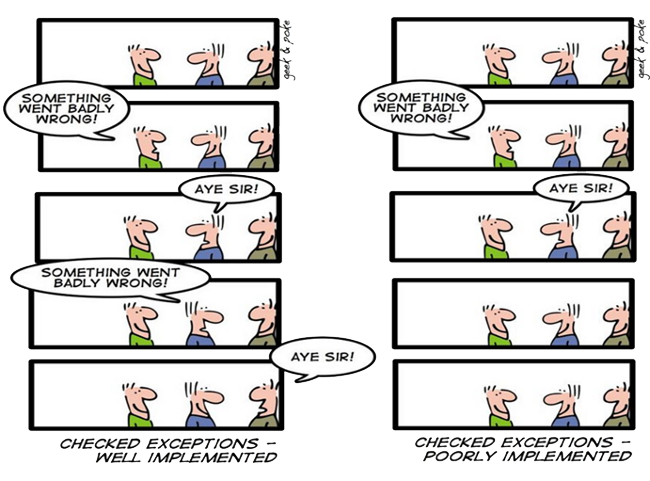
\includegraphics[height=0.8\textheight,]{\texDirectory/template/images/checked-exceptions.png}
	\end{figure}
\end{frame}

\begin{frame}[fragile]
	\frametitle{Exception Handling}
	\begin{block}{\texttt{throw} keyword}
		A method can throw an exception of particular type using the \texttt{throw} statement.
	\end{block}
	\begin{block}{Syntax}
		\begin{minted}[fontsize=\small,tabsize=8,linenos=none,firstnumber=1]{java}
throw new ExceptionType("customized message");
		\end{minted}
	\end{block}
\end{frame}

\begin{frame}[fragile]
	\frametitle{Exception Handling}
	\begin{block}{\texttt{Car.java} (v3.0) (Page 1)}
		\begin{minted}[fontsize=\small,tabsize=8,linenos,firstnumber=1]{java}
import java.util.Scanner;
public class Car {
	private int numPassengerMax;
	private int numPassenger;
	public Car(int numPassengerMax) {
		this.numPassenger = numPassengerMax;
	}
	public int getNumPassenger() {
		return numPassenger;
	}
		\end{minted}
	\end{block}
\end{frame}

\begin{frame}[fragile]
	\frametitle{Exception Handling}
	\begin{block}{\texttt{Car.java} (v3.0) (Page 2)}
		\begin{minted}[fontsize=\small,tabsize=8,linenos,firstnumber=11]{java}
	public void board() throws Exception {
		System.out.print("How many people to board? ");
		Scanner input = new Scanner(System.in);
		int num = input.nextInt();
		input.close();
		if (numPassenger + num <= numPassengerMax)
			numPassenger += num;
		else {
			throw new Exception("Exceeds seating capacity");
		}
	}
}
		\end{minted}
	\end{block}
\end{frame}

\begin{frame}[fragile]
	\frametitle{Exception Handling}
	\begin{block}{\texttt{CarTest.java} (v3.0)}
		\begin{minted}[fontsize=\small,tabsize=8,linenos,firstnumber=1]{java}
import java.util.InputMismatchException;
public class CarTest {
	public static void main(String[] args) {
		Car car1 = new Car(4);
		try {
			car1.board();
		}
		catch (InputMismatchException e) {
			System.out.println("Invalid input.");
		}
		catch (Exception e) {
			System.out.println("Bad response.");
			System.out.println(e.getMessage());
		}
	}
}
		\end{minted}
	\end{block}
\end{frame}

\begin{frame}[fragile]
	\frametitle{Exception Handling}
	\begin{block}{Problem Statement}
		It is not a good practice to throw exceptions of a type known to JVM for conditions considered exceptional only by programmer.
	\end{block}
	\begin{block}{Proposed Solution}
		Create a new customized exception class
	\end{block}
\end{frame}

\begin{frame}[fragile]
	\frametitle{Exception Handling}
	\begin{block}{\texttt{CarCapacityException.java}}
		\begin{minted}[fontsize=\small,tabsize=8,linenos,firstnumber=1]{java}
@SuppressWarnings("serial")
public class CarCapacityException extends Exception {
	public CarCapacityException() {}
	public String getMessage() {
		return "Exceeds seating capacity.";
	}
}
		\end{minted}
	\end{block}
\end{frame}

\begin{frame}[fragile]
	\frametitle{Exception Handling}
	\begin{block}{\texttt{Car.java} (v4.0) (Page 1)}
		\begin{minted}[fontsize=\small,tabsize=8,linenos,firstnumber=1]{java}
import java.util.Scanner;
public class Car {
	private int numPassengerMax;
	private int numPassenger;
	public Car(int numPassengerMax) {
		this.numPassenger = numPassengerMax;
	}
	public int getNumPassenger() {
		return numPassenger;
	}
		\end{minted}
	\end{block}
\end{frame}

\begin{frame}[fragile]
	\frametitle{Exception Handling}
	\begin{block}{\texttt{Car.java} (v4.0) (Page 2)}
		\begin{minted}[fontsize=\small,tabsize=8,linenos,firstnumber=11]{java}
	public void board() throws CarCapacityException {
		System.out.print("How many people to board? ");
		Scanner input = new Scanner(System.in);
		int num = input.nextInt();
		input.close();
		if (numPassenger + num <= numPassengerMax)
			numPassenger += num;
		else {
			throw new CarCapacityException();
		}
	}
}
		\end{minted}
	\end{block}
\end{frame}

\begin{frame}[fragile]
	\frametitle{Exception Handling}
	\begin{block}{\texttt{CarTest.java} (v4.0)}
		\begin{minted}[fontsize=\small,tabsize=8,linenos,firstnumber=1]{java}
public class CarTest {
	public static void main(String[] args) {
		Car car1 = new Car(4);
		try {
			car1.board();
		}
		catch (InputMismatchException e) {
			System.out.println("Invalid input.");
		}
		catch (Exception e) {
			System.out.println("Bad response.");
			System.out.println(e.getMessage());
		}
	}
}
		\end{minted}
	\end{block}
\end{frame}

\begin{frame}[fragile]
	\frametitle{Exception Handling}
	\begin{figure}
		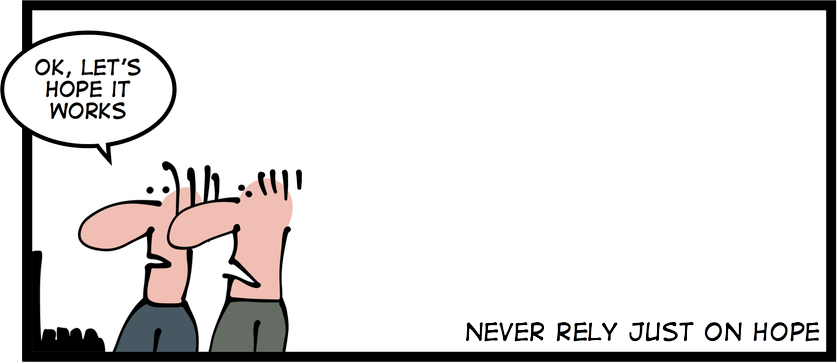
\includegraphics[width=\textwidth]{\texDirectory/template/images/hope1.png}
	\end{figure}
\end{frame}

\begin{frame}[fragile]
	\frametitle{Exception Handling}
	\begin{figure}
		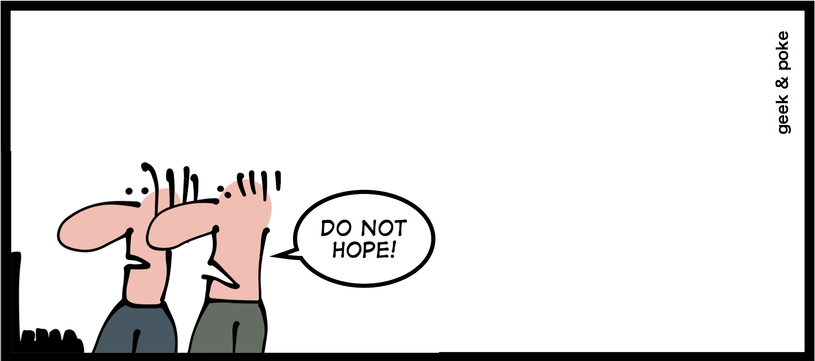
\includegraphics[width=\textwidth]{\texDirectory/template/images/hope2.png}
	\end{figure}
\end{frame}

\begin{frame}[fragile]
	\frametitle{Exception Handling}
	\begin{figure}
		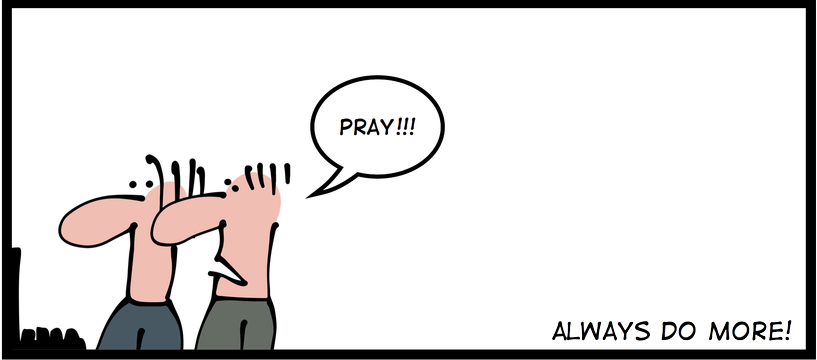
\includegraphics[width=\textwidth]{\texDirectory/template/images/hope3.png}
	\end{figure}
\end{frame}

\plain{}{Keep Calm\\and\\Enjoy Programming}

\end{document}
